\documentclass[11pt,titlepage]{article}
%\usepackage{amsmath}
%\usepackage{amsfonts}
%\usepackage{amssymb}
%\usepackage{algorithm}
%\usepackage{algorithmic} 
%
%\usepackage{theorem}
%\usepackage{graphicx}
%
%\usepackage[cp1250]{inputenc}
%\usepackage[T1]{fontenc}
%\usepackage[english]{babel}
%\usepackage[MeX]{polski}
%
%\usepackage{makeidx}
%\usepackage{listings}
%\usepackage{url}
%\usepackage{Here}

\usepackage{graphicx}
\usepackage{graphics}
\usepackage{epsfig}
\usepackage{amsmath}
\usepackage{amssymb}
\usepackage{amsthm}
\usepackage{booktabs}
\usepackage{stmaryrd}
\usepackage{url}
\usepackage{longtable}
\usepackage[figuresright]{rotating}

%\usepackage[MeX]{polski}
%\usepackage[cp1250]{inputenc}


%\usepackage[latin2]{inputenc}
\usepackage[english]{babel}
\usepackage[utf8]{inputenc}
\usepackage[T1]{fontenc}
\usepackage{geometry}
\usepackage{pslatex}
\usepackage{ulem}

\usepackage{lipsum}
\usepackage{amsmath}               
  {
      \theoremstyle{plain}
      \newtheorem{assumption}{Assumption}
  }
\usepackage{listings}
\usepackage{url}
\usepackage{Here}

\usepackage{color}
\definecolor{szary}{gray}{0.6}% jasnoszary

\setlength{\textwidth}{400pt}
\lstset{numbers=left,
			numberstyle=\tiny, 
			basicstyle=\scriptsize\ttfamily, 
			breaklines=true, 
			captionpos=b, 
			tabsize=2}

\usepackage[ruled,vlined,linesnumbered]{algorithm2e}


\selectlanguage{english}

%\vfuzz2pt % Don't report over-full v-boxes if over-edge is small
%\hfuzz2pt % Don't report over-full h-boxes if over-edge is small


\newcommand{\RR}{\mathbb{R}}
\newcommand{\NN}{\mathbb{N}}
\newcommand{\QQ}{\mathbb{Q}}
\newcommand{\ZZ}{\mathbb{Z}}
\newcommand{\TAB}{\hspace{0.50cm}}
\newcommand{\IFF}{\leftrightarrow}
\newcommand{\IMP}{\rightarrow}

\newtheorem{theorem}{Twierdzenie}[section]
\newtheorem{lemma}{Lemat}[section]
\newtheorem{example}{Przyk³ad}[section]
\newtheorem{corollary}{Wniosek}[section]
\newtheorem{definition}{Definicja}[section]

%\newenvironment{proof}{\par\noindent {\bf Dowód.}}
%{\begin{flushright} \vspace*{-6mm}\mbox{$\Box$} \end{flushright}}
%
%\newenvironment{remark}{\bigskip \par\noindent\begin{small}{\bf Uwaga.}}
%                       {\vspace*{4mm}\end{small}}
%
%\newenvironment{prog}{\par\noindent \sf
%\begin{tabbing}xx\= xx \= xx\= xx\= \kill}
%{\end{tabbing} \rm}


\makeindex

\begin{document}

\pagestyle{empty}

\begin{titlepage}
\vspace*{\fill}
\begin{center}
\begin{picture}(300,510)
  \put( 10,520){\makebox(0,0)[l]{\large \bf \textsc{Faculty of Fundamental Problems of Technology}}}
  \put( 10,500){\makebox(0,0)[l]{\large \bf \textsc{Wrocław University of Technology}}}
  \put( 10,280){\makebox(0,0)[l]{\Huge  \bf \textsc{
  Channels alternative to WiFi in }}}
  \put( 10,260){\makebox(0,0)[l]{\Huge \bf \textsc{
  Authenticated Key Establishment }}}
  \put( 10,240){\makebox(0,0)[l]{\Huge \bf \textsc{
  protocols for mobile devices}}}
  \put(100,200){\makebox(0,0)[l]{\large     \textsc{Paweł Kędzia}}}

  \put(170, 80){\makebox(0,0)[l]{\large  {In partial fulfillment of the requirements}}}
  \put(170, 60){\makebox(0,0)[l]{\large  {for the degree of Master of Engineering}}}
  \put(170, 40){\makebox(0,0)[l]{\large  { }}}
  \put(170, 20){\makebox(0,0)[l]{\large  {Thesis Supervisor}}}
  \put(170, 0){\makebox(0,0)[l]{\large  {dr inż. Łukasza Krzywieckiego}}}
  \put(100,-80){\makebox(0,0)[bl]{\large \bf \textsc{Wrocław 2010}}}
\end{picture}
\end{center}
\vspace*{\fill}
\end{titlepage}

\tableofcontents

\newpage

\pagestyle{headings}

\section{Introduction}

The goal of the dissertation is to analyze the usability of channels alternative to WiFi in Authenticated Key Establishment (AKE) protocols for mobile devices. Nowadays, more often mobile phones are used to sending secret data. Every this kind of device has embedded speaker and microphone therefore we want to check whether is possible to establish session key using just sound waves.

\vspace{5mm}

Mobile devices to transfer data mainly use Internet. Disadvantage of this method is that network not always is available. In that case one can still transmit data using some another embedded components like IrDA, Bluetooth or NFC. Unfortunately, not every device has these kind of accessories implemented. However, basis of handhelds is to have embedded speaker and microphone. That is why, in this dissertation, to communication between devices were chosen audio channel. Availability audio appliance and a lot of uses of this solution are main advantages. Furthermore receiver as like sender do not need to known each other (unlike Bluetooth) before starting the communication. Sender just starts to transmit data and receiver in the same time listens broadcast.

\vspace{5mm}

To authentication and key agreement between mobile devices was chosen Anonymous Mutual Authentication (AMA) protocol \cite{AMA}. AMA is symmetric, which means  participants execute the same operation (with some little difference in order of operations). One of
the advantage of this protocol eases implementation on resource limited devices. It was originally designed for authenticating electronic documents, it proved to be portable.

\vspace{5mm}

Application created on Android system will serve as proof of concept. There are application which use sound channel to exchange data, but none of them are used to establishing session keys. To use our application there is need just mobile phone/smartphone with software Android ( version 4.1.2 or higher ), working speaker and microphone, of course.

\vspace{5mm}

The first section focus on analysis of the problem. It explains principal issues used to create the application. It consists some information about security problem and necessary definitions to create sound channel. In the next chapter is described design of prototype. What was used, how application work etc. Then are shown results of test.


\subsection{Problem}
The problem is secure exchange keys between two parties, which have no knowledge of each other, in insecure, unreliable environment e.g. susceptible to eavesdropping.

\vspace{5mm}

The first known answer on this problem was published by Witfield Diffie and Martin Hellman. They have showed method to key exchange which is called Diffie-Hellman. Its strength and immunity to eavesdropping is based on Discrete Logarithm Problem. Existing computers are not able to compute session key from eavesdropped protocol transcript in reasonable amount of time.

\vspace{5mm}

Mentioned method is secure against eavesdropping, however it does not authenticate both parties to each other and thus does not guarantee security when adversary can take control over the channel in which the key establishment is being performed. Adversary, taking control over the channel, can perform Man-In-The-Middle-Attack (MITMA). MITMA is that, the adversary try to make some kind of connection with participants of protocol, being not detected. He can manipulate the communication pretending to be one of the party, changing or sending own messages, making them to believe that they are still talking to each other. The goal of these processes is obtain secrete key by attacker and thus decrypt and even modify all messages exchanged between parties.

\vspace{5mm}

To exchange data are used mainly electromagnetic radiation channels like Bluetooth, IRDa or Internet. We have wanted to check another options to exchanging data between devices, which does not use electromagnetic radiation. We have decided to study sound channel.


\subsection{Authenticated Key Agreement}

Authenticated Key Agreement Protocols base on public key cryptography and trusted authorities which are the most common solution being used. In public key cryptography are required two separate keys, where one is private and second one is public.

\vspace{5mm}

AKE protocols have to ensure that attacker can not obtain any information about session key from the protocol transcript. AKE protocols have to be resistant to exposed session transcript. Adversary should not be able to taking control over the communication channel having this knowledge.

\subsection{Out-of-band channel}
Beyond the security of AKE protocol, we wanted to study not typical communication channel to establish session key, which could hinder the manipulation in protocol transcript.

\vspace{5mm}

During the secure exchange data are needed two channels for communication between two parties. First channel, to establish session keys, should be difficult to eavesdrop and taking over control for adversary. The second channel can be insecure because established session key should ensure that content of protected data intended for one of the parties can be encrypt only by the party participated in protocol. For the key establishment, in our work, was chosen sound channel. We are aware there exist a lot of different type of microphone which are able to eavesdropping the sound waves. However, we will introduce some methods which could hinder in activity of attacker. The second channel for secure communication is wireless.


\subsection{AKE in out of-band channel}
Every mobile device have speaker and microphone. That is why the sound channel seems a reasonable choice as an out-of-band key establishment channel for mobile devices. Internet is not always available, so using this type of channel could be good alternative. Devices are still improving, hence speakers and microphones have better quality with each next generation. This paper is proof of concept and shows that it is possible to use this channel, at least partially, in these kind of applications. Each of the authenticating parties sequentially use their microphones and speaker to exchange data.


\subsection{Related work}
There are several ways to establish key. To prevent MITM attacks both parties have to authenticate to each other. There are many solutions that address this problem. One is to use shared secret password which prevents MITM as in EKE protocol \cite{EKE}. It was refined by many researches \cite{EKE, EKE2}. The requirement of pre-shared password between the parties might be impractical in many scenarios. There is also a family of Authenticated Key Agreement protocols (AKE) like Sigma \cite{sign_mac}, HMQV \cite{HMQV}, KEA \cite{KEA}, CMQV \cite{CMQV}, Naxos and Naxos pls like protocols \cite{AMA, NAXOS}. The security requirements and security model definition in AKE protocols were proposed by Cenetti and Krawczyk in \cite{cankraw1, cankraw2}. In this paper we focus on usage of optical channel for authentication thus in practice any key agreement protocol that is secure against active adversary could be used. Out-of-band channels for key agreement protocols are discussed in [2, 3, 4, 16].

\section{Analysis of the problem}

In this section we will focus on problem of establishing secure connection in insecure channel between two parties. At first the parties need to authenticate each other and then create common session key, which will be needed to symmetric encryption of the communication. We describe the adversarial model where is assumed that each of the parties secretly holds a long-term private key that enables unique authentication of this party. There is also a trusted mechanism for binding identities with public keys. The private and public key with proper length are bounded in such way that obtain private key from public key is very hard to do. The communication channel can be completely controlled by an adversary that can intercept, delete, delay, modify or inject messages at will. There is a relation between the requirements of the security model and a well-defined attack scenario. In the second part of this section are described necessary issues to create sound channel.

\subsection{Anonymous Mutual Authentication}
To establish session keys we used in our prototype Anonymous Mutual Authentication protocol which base on Diffie-Hellman key exchange. 

\vspace{5mm}

AMA originally was designed to anonymous authenticate between smart cards. Is characterized by properties:
\begin{itemize}
\item Forward Security - if long term keys of one of the authenticating parties compromised then established session key does not reveal.
\item Simultability - is possible to create protocol transcript between parties without interacting with them
\item Undetectability - having protocol transcript one cannot confirm that process really took place
\item Privacy - eavesdropping adversary cannot tell about identity of parties performing the protocol
\item Deniability - no one of the parties cannot convince third party that he participate in protocol.
\end{itemize}

\begin{figure}[H]
	\centering
	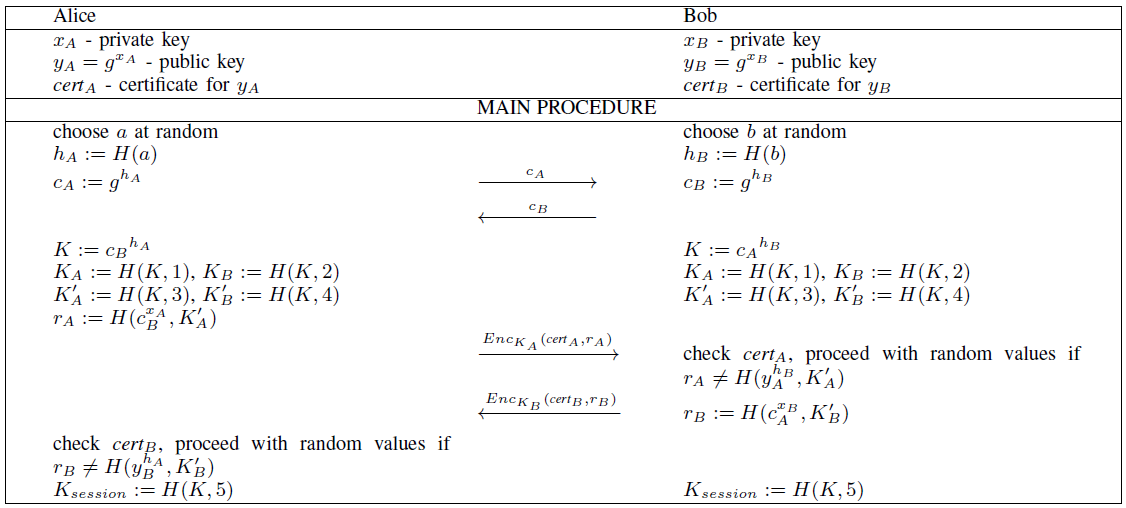
\includegraphics[width=1.2\textwidth]{img/AMA_protocol}
	\caption{Protocol description - Anonymous Mutual Authentication. Figure from source \cite{AMA}.}
	\label{fig:F8}
\end{figure}

Scheme of protocol is shown at the \ref{fig:F8}. In scheme are use the following notation:
\begin{itemize}
\item \textit{Enc} is a symmetric encryption function. \textit{$Enc_K(M)$} means encryption of $M$ using key $K$. 
\item \textit{H} is a cryptographic hash function. 
\item For confirming public keys are using digital certificates and public key infrastructure (PKI).
\end{itemize}

AMA is defined in a cyclic group G where Computational Diffie-Hellman Problem (CDH) is hard

\begin{assumption}
Given a cyclic group G with order $q$, and ($g$,$g^a$,$g^b$) where $g$ us a random generator of $G$, and ($a$,$b$) where chosen randomly from the set {0,1,...,$q-1$} it is computationally intractable to compute the value $g^{ab}$.
\end{assumption}

At the beginning, parties (Alice and Bob) generate their private key - $x_A$ (respectively, $x_B$) and public key $y_A = g^{x_A}$ (respectively, $y_A$). Then parties generate their ephemeral keys. Private is $h_A$ := $H(a)$ (where $a$ is a random number) (respectively $h_B$, $b$) and public ephemeral key $c_A$ := $g^{h_A}$ (respectively $c_B$). Then participants exchange their ephemeral keys, based on Diffie-Hellman key exchange. Note that in this phase parties do not exchange any identity information.

\vspace{5mm}

When parties obtain ephemeral public key of another party, they start compute master
key $K$. Four different one-time keys are establish by hashing $K$ and numeric parameter - different for each one-time key.

\vspace{5mm}

To authentication, parties encrypt their certificates $cert_A$ and $cert_B$ and the challenge values $r_A$ and $r_B$ which are the hash of two keys. Authenticated party is raising ephemeral public key $c_B$ (respectively, $c_A$) to power of private key $x_A$ (respectively, $x_B$). Verifier compute the same value without private key but with the discrete logarithm of $c_A$ (respectively, $c_B$) which is $y^{h_B}$ (respectively, $y^{h_A}$ ). If the compared values are equal then $K_{session}$ is the hash of master key $K$ and new number parameter.

\vspace{5mm}

This protocol is proved to be secure under Random Oracle Model (ROM) for the used
hash function $H$. In ROM, hash function $H$ is modeled as an oracle $\mathcal{O}_H$. For a query $x$, oracle responds $y$ if in internal table $T$ exist entry ($x$, $y$). If there is no such an entry for $x$, then $\mathcal{O}_H$ selects $y$ at random, creates entry ($x$, $y$) is in $T$ and answers $y$. In this model the only available operation concerning hash function $H$ is asking for values for concrete arguments. Hence, having value $y$ the only way to get $x$ = $H^{-1}(y)$ is to remember it from a previous query or ask a query with new $x$ and get $y$ by accident. Security proof of symmetric encryption is shown by series of games, for more details see \cite{AMA}. 

\vspace{5mm}

The practical part of this paper was to implement AMA on mobile devices as to our best knowledge there is no practical implementation of AMA for smartphones.

\newpage
\begin{table}[H]
\caption{Scheme of protocol used in devices.}
\begin{center}

\begin{tabular}{ p{4cm} p{5cm} p{4cm}}
\textsf{\LARGE Alice} & & \textsf{\LARGE Bob} \\
\hline
\textsf{\newline\textbf{\small Starting screen} \newline
\newline
\footnotesize Alice starts the protocol as initializator}& \raisebox{-\totalheight}{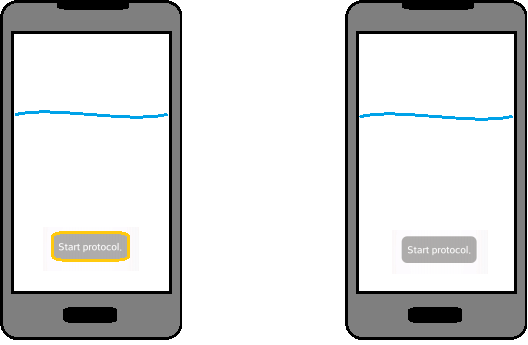
\includegraphics[width=0.27\textwidth, height=27mm]{img/couple.png}} & \textsf{\newline\textbf{\small Starting screen} \newline \newline
\footnotesize Bob starts protocol as receiver.} \\

\textsf{\newline\textbf{\small Send ephemeral key} \newline
\newline
\footnotesize Alice generates ephemeral key, encodes and start sending it by speaker.}&\raisebox{-\totalheight}{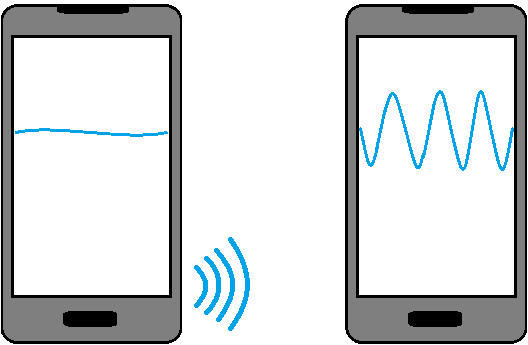
\includegraphics[width=0.27\textwidth, height=27mm]{img/signal1.png}}&\textsf{\newline\textbf{\small Receive ephemeral key} \newline
\newline
\footnotesize Bob receives ephemeral key using microphone.} \\

\textsf{\newline\textbf{\small Receive ephemeral key } \newline
\newline
\footnotesize Alice receives ephemeral key using microphone. }&\raisebox{-\totalheight}{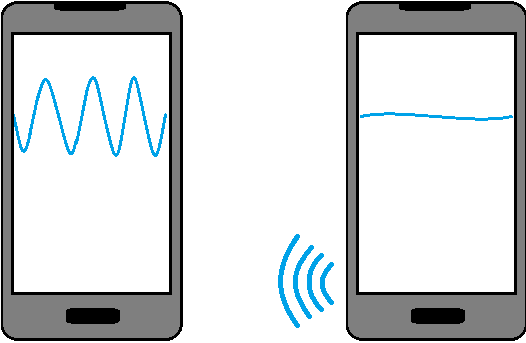
\includegraphics[width=0.27\textwidth, height=27mm]{img/second_side.png}}&\textsf{\newline\textbf{\small Send ephemeral key} \newline
\newline
\footnotesize Bob generates ephemeral key, encodes and start sending it by speaker.} \\

\textsf{\newline\textbf{\small Send encrypted authentication data } \newline
\newline
\footnotesize Alice uses her and Bob's ephemeral keys to compute authentication data, encrypts it and sends by speaker. }&\raisebox{-\totalheight}{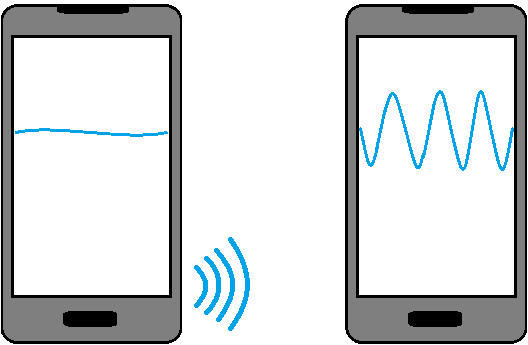
\includegraphics[width=0.27\textwidth, height=27mm]{img/signal1.png}}&\textsf{\newline\textbf{\small Receive and decrypt authentication data} \newline
\newline
\footnotesize Bob receives and decrypts Alices authentication data.} \\

\textsf{\newline\textbf{\small Receive and decrypt authentication data } \newline
\newline
\footnotesize Alice receives and decrypts Bobs authentication data. If it's not valid, she aborts the protocol. }&\raisebox{-\totalheight}{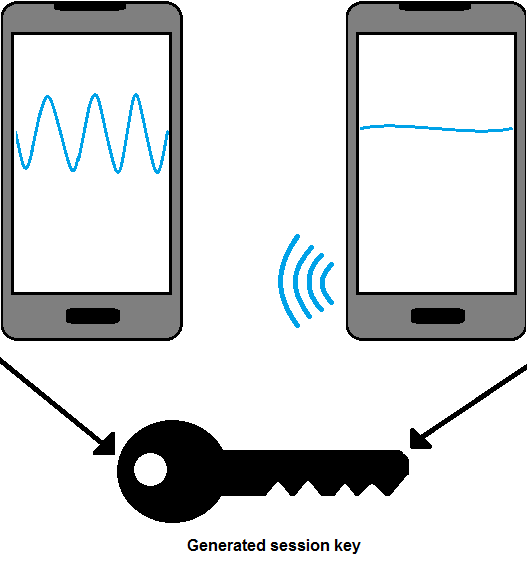
\includegraphics[width=0.27\textwidth, height=50mm]{img/session_key_est.png}}&\textsf{\newline\textbf{\small Send encrypted authentication data} \newline
\newline
\footnotesize Bob verifies authentication data received from Alice. If it's
valid, he generates his authentication data and send it by microphone. If data is not valid, Bob aborts the protocol.}
\end{tabular}
\end{center}
\end{table}
\subsection{Sound}
Sound is acoustic wave propagating in different substances such as water, air (so called vibrating wire). These are waves which cause auditory sensation and at the same time in appropriate amplitude and frequency are not detected by human organ of hearing. Sound to spread need to has some medium, that is why not propagate in vacuum. Furthermore, sound is longitudinal waves, which means that particles of the medium is in the same direction as the direction of travel of the wave.



\begin{center}
	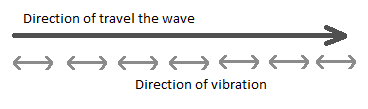
\includegraphics{img/longitudinal_wave}
\end{center}
\subsubsection{Frequency}
Audio frequency is measured in hertz (Hz), where 1 Hz means one cycle per second. Below figures show graphs of audio frequency 1 Hz and 5 Hz.

\begin{center}
	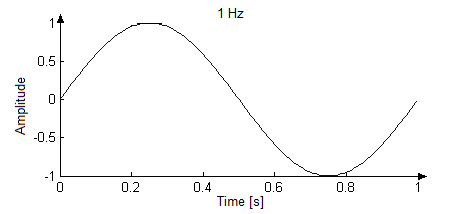
\includegraphics[width=0.45\textwidth]{img/frequency_1Hz}
	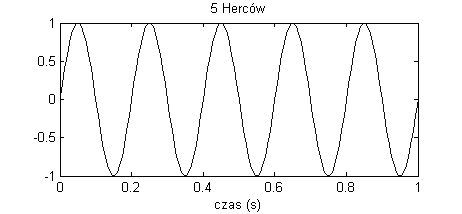
\includegraphics[width=0.45\textwidth]{img/frequency_5Hz}
\end{center}

Exist three division of sound as to frequency:
\begin{itemize}
	\item Infrasound - frequency is lower than 16~Hz.
	\item Hearable sound - frequency is greater than 16~Hz and lower than 20~kHz.
	\item Ultrasound - frequency is greater than 20~kHz.
	\item Hipersound - frequency is greater than 10~GHz.
\end{itemize}

Frequency specify also pitch of sound. A high frequency sound wave corresponds to a high pitch sound and low frequency sound wave corresponds to a low pitch sound.

\subsubsection{Sound intensity}
Loudness of the sound is dependent to his intensity. It is expressed by $W/m^2$ unit. This is ratio the power of the acoustic wave to surface area to which wave energy falls perpendicular during 1 second \cite{sound_intensity}. Human's ear works in such way that doubling intensity of sound, do not cause that human hear it two times louder. Human hears its logarithmized value. Logarithmized measure of sound intensity is called sound intensity level. Is measured in decibels and is given by \cite{decibels}:
\begin{equation}
	L = 10\log_{10}(\frac{I}{I_o})  [dB],
\end{equation}
where:
\begin{itemize}
	\item $L$ - Sound intensity level.
	\item $I$ - Sound intensity.
	\item $I_o$ - Contractual value of the intensity which determines hearing range, which is $10^{-12}\frac{W}{m^2}.$
\end{itemize}
\subsubsection{Speed of sound}

Speed of sound depends on center through which wave passes. Influence on speed has also temperature of the center. The slowest moves in the flue. In the air with $20^o$ temperature reach in  approximation 343 m/s (1230 km/h). In water with the same temperature speed is 1482 m/s (5335 km/h). The fastest sound spread in solid. For example in steel reach about 5960 m/s (21460 km/h) \cite{sound_speed}.

\subsubsection{Ultrasounds}
The present app largely, to sending data, uses ultrasound. Ultrasound are sound waves, which are inaudible for human, on the grounds of their too high frequency. Have adopted that ultrasounds starts from 20 kHz, but really everything depends on how good hearing human has. Children hear the highest frequencies. Increasing age the upper limit of hearing descend \cite{limit_sound}. Ultrasounds end at frequencies  of several GHz, where hipersounds start. Contractual it is 10 GHz.  Ultrasounds have many applications. Using them one can detect objects and specify distance to them. Are used in medicine where whereby ultrasonography (USG) we can find not available for human eye diseases, watching e.g. internal organs. 

\subsubsection{Fourier transform}
By Fourier transform one can change function $f(x)$ in time domain to $F(s)$ in frequency domain. In other words, distribute the function $f(x)$ to series of periodic functions, in such way that show how frequencies consist of the function $f(x)$. The formula for the Fourier transform looks as fallows:

\begin{equation}
	F(s) = \int\limits^\infty_{-\infty} f(x) e^{-i2\pi xs} dx.
\end{equation}

Sum of three functions with frequencies 3 Hz 7 Hz and 11 Hz on a graph:
\begin{figure}[H]
	\centering
	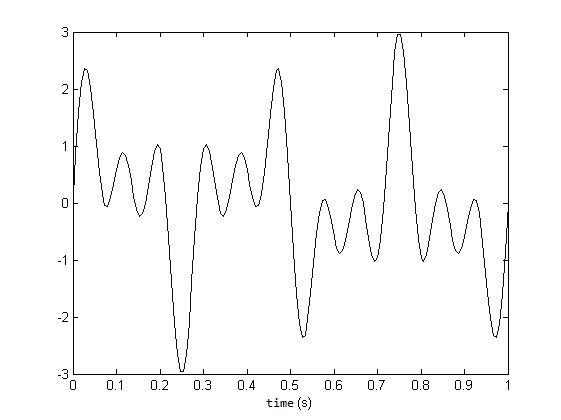
\includegraphics[width=0.5\textwidth]{img/sines}
	\caption{$f(x) = \sin(2\pi \cdot 3t)+\sin(2 \pi \cdot 7 t)+\sin(2  \pi \cdot 11  t)$, where t is current time.}
	\label{fig:F4}
\end{figure}

Passing function $f(x)$ from figure \ref{fig:F4} through Fourier transform we will get the following graphs:

\begin{figure}[H]
	\centering
	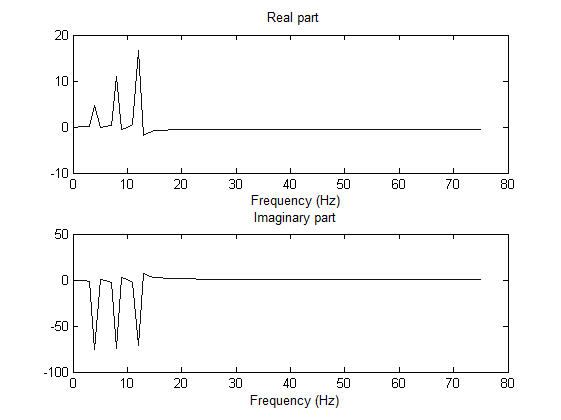
\includegraphics[width=0.65\textwidth]{img/both_real_imag}
	\caption{On the top real part results of Fourier transform, on the bottom imaginary part.}
	\label{fig:F5}
\end{figure}

As you can see on above figure, time domain was changed on frequency domain. On graphs are bigger values for frequencies which had summed functions.

\subsubsection{Discrete Fourier Transform}
Application analyzes periodically finite number of samples of sound. To converse to frequency domain is used Discrete Fourier transform (DFT). Inserted samples are in the form of complex numbers, but in practice used only real numbers. Output samples are complex numbers. The following graphs show continuous signal and discretized signal \cite{fourier}:

\begin{figure}[H]
	\centering
	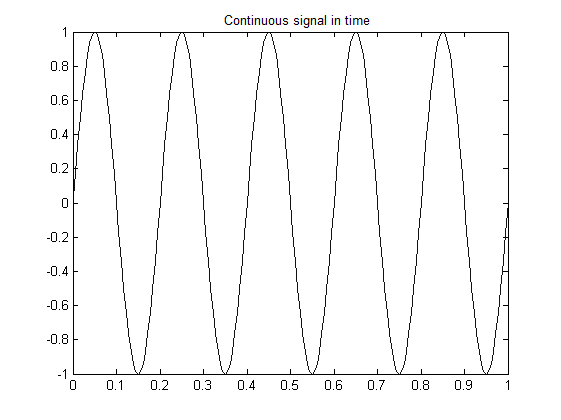
\includegraphics[width=0.6\textwidth]{img/continues}
	\caption{Continuous signal in duration 1 second.}
	\label{fig:F6}
\end{figure}

\begin{figure}[H]
	\centering
	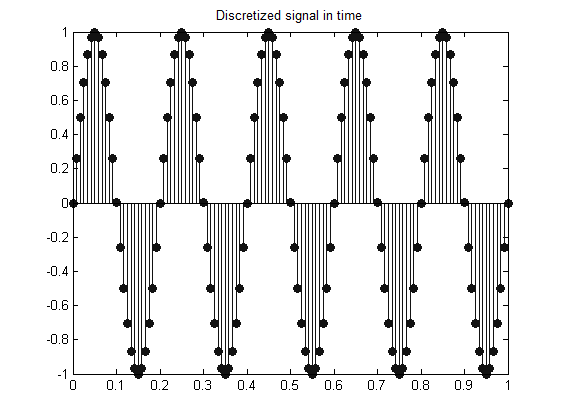
\includegraphics[width=0.6\textwidth]{img/descrete}
	\caption{Discretized signal in constant time period. In this case in 1 second are 121 samples.}
	\label{fig:F7}
\end{figure}

For $N$ signal samples $(x_0,x_1,x_2,...,x_{N-1})$, discrete Fourier transform gives series $X_k$ for $k = 0,1, 2, 3, ..., N-1$ using notation \cite{fourier}:
\begin{equation}
	X_k =  \sum\limits_{n=0}^{N-1} x_ne^{-i2\pi \frac{k}{N}n}.
\end{equation}
Computational complexity this notation is $O(N^2)$, because for $N$ elements $X_k$ series compute sum for $N$ samples \cite{fast_fourier}.

\subsubsection{Fast Fourier Transform}
Computational complexity of discrete Fourier transform is not enough to fast process more data. Therefore developed a lot of algorithms, which improve its calculation. Exist algorithms, which do discrete Fourier transform having computational complexity $O(NlogN)$, where for large number of data is significant improvement. They use design paradigm divide and conquer. Precursors of these solutions are James William Cooley and John Tukey, who elaborated first faster algorithm to compute DFT, known as fast Fourier transform (FFT). It is worth mentioning that FFT is not approximate value of DFT. FFT returns the same values but do this much faster.

\subsubsection{Hanning window}
Window functions are functions which are used with DFT. Often during process of DFT occur blur of spectrum, which mean that on the spectrum are seeing values for frequencies different than the real frequency of signal. To minimize this effect are used window functions. In time domain it is multiply every sample of signal by corresponding value of sample of window. The simplest window is rectangular window. Spectrum of this windowing is shown in \ref{fig:F9}
\begin{figure}[H]
	\centering
	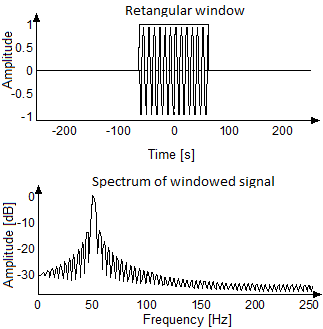
\includegraphics[width=0.6\textwidth]{img/rectangular_window}
	\caption{Rectangular window and its effect in spectrum of signal.}
	\label{fig:F9}
\end{figure}

\vspace{5mm}

In our protocol is used Hanning window which is defined by:
\begin{equation}
	 w(n) = 0.5 (1 - \cos\left(\frac{2 \pi n}{N - 1}\right)),
\end{equation}
\newline where $N$ - amount of analyzed samples, $n$ - nth sample. 

\vspace{5mm}

As one can see at figure \ref{fig:F10} the pitch is wider, hence is easier to determine the correct frequency.
\begin{figure}[H]
	\centering
	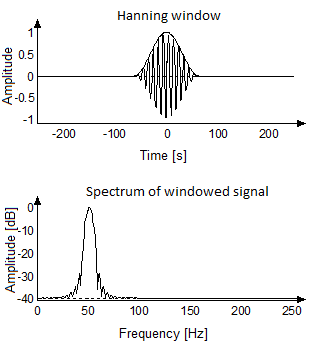
\includegraphics[width=0.6\textwidth]{img/hanning_window}
	\caption{Hanning window and its effect in spectrum of signal.}
	\label{fig:F10}
\end{figure}

\subsubsection{Pulse-Code Modulation}

Pulse-Code Modulation (PCM) is a method used to digitally represent sampled analog signals. PCM is based on representation of the instantaneous value of the signal (Sampling) at uniform intervals (sampling rate). The sampled analog data are represent by binary data. During the demodulation, sample rate should be at least two times greater that frequency of receiving analog signal (greater than the Nyquist frequency $f_s / 2$ ). This ensure that sampled values represent analog signal without errors. In our prototype sample rate is 44,1 kHz. The highest frequency which we use in application is about 20,5 kHz so 44,1 kHz is sufficient. 

\subsubsection{Doppler effect}
We introduce this phenomenon because of one of the possibility to prevent against effective
eavesdropping. Doppler effect is that the receiver get different frequency of wave from frequency which is generated by moving source relative to the receiver. The simplest example
is when ambulance with turn on siren is coming to us. Then we are receiving higher frequencies
from the emitted frequency. When ambulance is passing us then we hear the same
frequencies. When is moving away then we hear the lower frequencies. Observed frequency $f$ is given by:

\begin{equation}
	f = f_{0} \cdot \left(\frac {c}{c + v_{s}}\right),
\end{equation}
\begin{equation}
	f = f_{0} \cdot \left(\frac {c + v_{r}}{c}\right),
\end{equation}

where

\begin{itemize}
\item $f_0$ emitted frequency;
\item $c$ is the velocity of waves in the medium;
\item $v_r$ is the velocity of the receiver relative to the medium;
\item $v_s$ is the velocity of the source relative to the medium;
\end{itemize}

The formula (5) shows describe situation when source is moving when observer is stationary, but (6) in the opposite way. Both formulas can be combined into one:

\begin{equation}
	f = f_{0} \cdot \left(\frac {c + v_{r}}{c + v_{s}}\right).
\end{equation}

In our case authenticated parties are not moving relative to each other, but they can both moving relative to eavesdropper.

\subsection{Security Model}
There is no one ultimately defined security model for key exchange. However, we will recourse to the requirements as most fundamental for secure key exchange protocol which H. Krawczyk presents in \cite{sign_mac}.

\begin{itemize}
\item Authentication - each party participating in KE needs to uniquely verify identities of other authenticating party.
\item Consistency - two parties participating in KE, after establish of session key have to believe that were established common session key with party which participate in protocol. In other words, Alice has to believe that she established session key with Bob and Bob has to believe that he established session key with Alice.
\item Secrecy - if two honest parties established session key then third party should not be able to obtain information about this session key. Third party, which watching and interfering with the protocol run, should not be able to distinguish session key from a random key.
\end{itemize}

\subsubsection{Adversarial Model}
Is needed to consider scenario where adversary learns some secrete information from parties participant in protocol. The worst case is when adversary obtain the long term secrete key from one of the party. Having this key adversary can completely control this party and the party is consider corrupted. This lead to belows property of the KE protocol.

\begin{itemize}
\item Real-or-Random - this is some kind of game on which basic session key security is based. When uncorrupted parties with successful end the protocol then is determined bit $b$ at random. If $b=0$ the adversary get the real session key, if $b = 1$ he receives a random value with the same length as the key. Now adversary has to output his own bit $b'$. If $b' = b$ then adversary wins the game. When the adversary wins the game with probability $P = 1/2+\epsilon$, where $\epsilon$ is negligible function then the basis session key security is achieved.
\item Perfect Forward Secrecy (PFS) - is the property which ensure that adversary cannot learn session keys when one of the long-term private key is compromised in the future.
\end{itemize}

Above criteria ensure for key exchange protocol that they are resistant to attacks like known-key attacks and replay attacks \cite{cryptography}. For some KE protocols are needed additional requirements e.g. Identity protection - identities of authenticating parties cannot be learn by an adversary.

\subsection{Analysis of out-of-band channels}
There are a lot of techniques to transfer secret data between devices. The most popular are e.g. Bluetooth, IrDA or WiFi. These techniques use electromagnetic waves. To manipulating, changing or eavesdropping messages are needed devices which operates on electromagnetic radiation (e.g. bug in the phone). So it is worth to consider out-of-band channel which is not so commonly used as electromagnetic devices.

\vspace{5mm}

Safety channel could be, for example, two devices connected by wire. For the third party would be very difficult to eavesdrop the session. Attacker should be connected also to this wire but it would be visible for the other parties and easily to detect. Unfortunately, carrying additional cable every time when the parties want to establish session key is inconvenient.

\vspace{5mm}

The other possibility could be optical channel \cite{QRcode}. Sharing data using e.g. QR codes is also interesting way to authentication of devices. Attacker would have difficult task to manipulate shared data if e.g. two devices are covered by some walls. However, not every device has camera with appropriate quality that can read QR codes with appropriate big public keys.

\vspace{5mm}

Another way is to use vibrations \cite{vibrat}. New smartphones have installed sensor of vibration so it is possible to create such a communication channel. Attacker to manipulate this kind of channel has to generate own vibrations and it would be easily detected by authenticating parties.

\vspace{5mm}

Sound channel is also one of the options. Every mobile device has speaker and microphone, so we do not need to worry about no available Internet or that the other party has not installed Bluetooth or IrDA or even camera. Using ultrasounds, the signal will be not detected by humans ear. Additionally mobile phones cannot generate these waves with big intense, so transferring data should be done on small distance. Of course, sound channel could be easily to manipulate. Attacker with proper speaker can generate frequencies which could disturb the communication. However, he needs to be close to the authenticating parties if generated ultrasound has to be detected by party,s mobiles microphone or generate sound waves with big intense which could be audible for human. Additionally is worth to consider use this kind of channel mixing with another channel. For example, ephemeral keys will be sending by sound channel then encrypted values by Bluetooth.

\subsection{Proposed usage of out-of-band channel}

Lets assumed that Alice and Bob want to establish a secure connection between their mobile phones using sound channel. To be sure that every high frequency will be detected, they try to put their phone in a such way that microphone is as close as possible to speaker of the second phone and vice versa. Usually the speaker and microphone are set at the bottom of device, so mobile phones should be directed bottom to each other. To obtain session key is processed AKE protocol. After this process further exchange of data can be done by WiFi, because of the speed of transferring data which is higher. 

\vspace{5mm}

\begin{itemize}
\item Alice and Bob put their devices into the lead box. Both mobile phone are listening for the first sign. The first one which start generated sound wave will be initiator. For the best quality of transferring data mobiles should be directed bottom to each other no more than couple of millimeters.
\item Alice decided to be initiator of the protocol. She says "Start" to the little hole in the box and her phone, after recognized her voice, start sending first data.
\item Protocol is divided on couple of phase. First phase is sending ephemeral key by initiator (in our case by Alice) to the receiver. Each phase takes couple of seconds. Every data are encoded in sound waves with appropriate frequencies.
\item Bob's phone uses its microphone to obtain the data sent by Alice's device.
\item When phase is over, follow switch of the roles. Now Alice's phone will listening and Bob's phone sending data.
\item Alice's device will receiving and decode it.
\end{itemize}

Anonymous Mutual Chip Authentication (described in detail in section above) should ensure that even if some transferring data eavesdrop then adversary will do nothing with this data. Duration of the protocol is about 40 second - more information about duration and performance are described in section 5.

\subsection{Sound channel parameters}

Using Diffie-Hellman key exchange and asymmetric cryptography should be use the longest key length as possible. In NIST specification SP 800-131 is mentioned that recommended key length is 3072. However, in our prototype we used 1024 key length. The reason is low speed of transferring data, which is 200b/s. Decreasing time of sending one character had influence on analyzing received data. It have been taking too long time (frequency of getting data increased, so algorithm did not follow in analyze so much data in short time).

\vspace{5mm}

Sound channel is secured against active attacks. Adversary needs to be close to communicated party or he needs to generate ultrasound with high intense which can be detected by human, it would be heard as squeak.

\subsection{Enhance the project}
Lets imagine that Alice and Bob want to establish secure channel being far away from each other. They can authenticate each other using telephone line. Is possible to run application during the calling but the microphone receiving the signal is unavailable in the app. So to this experiment would be needed second pair of mobile phones which will be used as intermediary. Each intermediary phone should be set as handsfree because of loudness of sound. Authenticated phones should be apply as close as possible to intermediary phone. Now when intermediary phones established the connection, the authenticated devices can start the protocol, the sound signal will be transferring by telephone line. Device on the other side will be receiving the signal. 

\vspace{5mm}

Disadvantage in our protocol is speed of transferring data. In every 15 milliseconds are received samples which are put to the queue. Another process gets these samples and analyze them. For our test devices, receiving data in every 15 second was the most optimal method. Algorithm analyzing this data follow with computing, so in queue do not accumulate to much data. Decreasing period receiving data to 10 millisecond cause that decoder of sound did not keep up and outcome was sometimes couple of seconds after the last received character. To improve that is worth to considering client-server model. Mobile phone as a client gathering the data and send to the external server. Server with much more computing power could decode the data definitely faster and returns the result to the client. Server could do much more complex computing, hence the results would be with better precision.

\vspace{5mm}

For now the sound channel use bandwidth from 10,5 kHz to 20,25 kHz. For the reason please check section with Base64 conversion. These frequencies (especially below 19 kHz) could be audible for the most of the people (it sounds like squeaking). If we would want to exchange data using sound which is inaudible, we could use just simple binary representation. Sending data using 0 and 1 would be needed only two frequencies, so taking the highest as possible (for example 19,9 kHz and 20,10) would ensure that exchanging of data would be inaudible for the most people. Of course at the expense of length of sending data. It would be achievable also with hexadecimal representation. Would be needed to use bigger bandwidth than from binary representation but the length of data would be smaller.

\subsection{Microphones and speakers in mobile devices}
Specification of this appliances are very different and depends on devices. During the tests could be seen that microphone from more expensive SAMSUNG Galaxy Tab is better than microphone from LG Swift L9. SAMSUNG could detect higher frequency. However, microphone from LG Swift L9 was completely enough to registered sufficiently large frequencies. Speakers also are a little different, but they have no problem to generate opportunely frequencies.



\subsection{Security analysis}
The key exchange protocol is considered to be secured on the assumptions that underlying problems are hard e.g. factorization, discrete logarithm, computational Diffie-Hellman etc. One interesting question is what happens if those assumptions are false. Lets imagine an adversary with super efficient quantum computer that is capable of solving the above problems in reasonable time.

\vspace{5mm}

The adversary can have different powers over the communication channel. In the following paragraphs we will discuss different powers of the adversary and their influence over the security of the protocol.

\vspace{5mm}

The security analysis below does not include security proofs of AMA but the different aspects of an adversary capturing the transmission if he was able to break the aforementioned assumptions.

\subsubsection{No access to protocol transcript}
At first the adversary might not be able to eavesdrop the transcript of the protocol at all e.g. in environment where capturing the communication requires sufficient distance to obtain sound signal from the authenticating devices. In that case there are not a lot of requirements for the key exchange protocol being used.

\vspace{5mm}

This case is trivial as we can imagine a very simple game in which two parties are hidden from an adversary and he has to guess whether the parties performed a key exchange protocol. Without access to the messages exchanged between the parties, an adversary can only guess with probability $P = \frac{1}{2}$ if the parties performed the protocol. As a consequence he cannot win the "Real-or-Random" game concerning the session key in underlying CK or eCK models for the chosen AKE protocol \cite{key_exchange, efficient_eck, security_canetti_krawczyk}. Similarly, using the same reasoning, the adversary cannot guess the identities of parties mutually authenticating in the protocol. 

\vspace{5mm}

However in practice it is possible for an adversary to partially eavesdrop the communication between devices.

\subsubsection{Partial access to protocol transcript}

Partial access to protocol transcript in sound channel will be depends on many factors. At first microphone has to have appropriate sensitivity level. Sensitivity level is given by:

\begin{equation}
	L_m = 20 lg(\frac{M}{M_0})dB,
\end{equation}

where $M$ is sensitivity [mV/Pa] and $M_0$ is the 1000 mV/Pa (1 V/Pa) reference output ratio. Microphone sensitivity $M$ depends also on frequency and the angle of incidence. The important role of receiving signal have speakers generating this signal. Sensitivity level of speaker is given by: 

\begin{equation}
	L_s = 10 lg(\frac{p_A}{p_0})dB,
\end{equation}

where $p_A$ is sound pressure generated by speaker powered 1V*A, $p_0$ is a reference pressure which has value $2*10^{-5}$ Pa. Frequency also has influence on sensitivity level of speaker. The next thing which should be consider is distance microphone from speaker. Too big distance and too low sensitivity of microphone could causing that microphone will not able to gain sounds wave or at least some frequencies. Sound pressure decreases proportionally with increase of distance. So when sound level $L_{1}$ is measured at a distance $r_1$, the sound level $L_2$ at the distance $r_2$ is given by:

\begin{equation}
	L_2 = L_1 + 20 lg (\frac{r_1}{r_2}).
\end{equation}

These factors contribute to some probability $\bar{p}$ that adversary and participants will have this type of devices satisfying the conditions. Otherwise, adversary not being able to receive all frequencies he will gain transcript with data having no sense.


\subsubsection{Full access to protocol transcript}
Imagine that an adversary uses some kind of microphone with high sensitivity so he can capture all communication between authenticating devices. As mentioned in the previous section in order to secure against eavesdropping the key exchange protocol must use difficulty to inverse problems like the discrete logarithm problem used in the Diffie-Hellman key exchange scheme.

\subsubsection{Possible vectors of attack on a sound channel}
There are two ways to attack the sound channel. The first one is trying to generate sound wave which can drown or change sending data by one of the authenticate parties. Additionally one can in some ways force microphone to gaining frequencies in another bandwidth. Soundproofing box or case could hinder these type of attack. The second possibility to prevent against eavesdropping attack is using phenomenon of Doppler effect. Lets imagine that two mobile devices are put on some kind of tape. This tape in appropriate high speed starts randomly moving in different ways. Authenticated devices will be in the same position relative to each other but they will be constantly on the move relative to third party. Doppler effect will cause that eavesdropper will receive different frequencies than generating. For more details of Doppler effect see the section "Doppler effect" above. Good solution would be mixing the channel. For example, first phase (exchanging ephemeral keys) would be process by out-of-band channel but second phase (encrypted identity information) by commonly used radiation channel (WiFi, Bluetooth).

\subsubsection{Manipulating speaker}
One of the vector attack is manipulating of the speaker. Assume that adversary want to run malicious program which take control over the speaker. He can generates waves what he wants, hence he can send malicious data and encryption due to which he can learn something about the protocol. System has to ensure that during process of key exchange any kind of background application cannot interrupt this. Android ensure security in that way but do not forget about different type of viruses. Unfortunately we do not have influence on this. Manipulation from external is based on using additionally speaker which will generate sound in used bandwidth. This method could mislead of the receiving microphone. It would be easy to disturb the signal but then recorder will gain data with no sense. Attacker would has to start generate sound in perfect time with appropriate intense. Large distance could causing that would be necessary some calculation about speed of sound. High intense (which would be needed if microphone would has to receive high frequencies from distance) could cause that signal would be audible for human, hence attacker could be exposed. Inserting authenticated parties to some soundproofing box could minimize effectiveness of these methods of attacks.

\subsubsection{Manipulating microphone}
Manipulation of microphone would be possible only if attacker would have access to the application. He could e.g. reduce or increase bandwidth of frequencies. Adversary could totally change the bandwidth, outside of the know range for authenticated parties and at the same time generate his sound waves in chosen bandwidth.

\subsubsection{Eavesdropping}
There are exist a lot of devices to eavesdropping. One of the example is microphone with high sensitivity which allow to eavesdrop the sounds even from a large distance e.g. parabolic or shotgun  microphone. To gain ultrasounds for eavesdropper would be useful instrument detecting ultrasonics from bats. The next one is using laser \cite{laser_mic}. The special laser is a transmitter and the infrared measure of surface vibration. This method also allows to gain data from a large distance. However beyond the soundproofing boxes is worth to use phenomenon of Doppler effect. Constantly moving devices will cause that emitted frequencies will be different than observer will registered. 

\subsubsection{Malicious implementation}
An adversary could try to swap a genuine application for the key exchange on the authenticating device with a malicious one and thus gain the session key. To ensure both parties that they use genuine software, it should be signed with a certificate of a trusted authority and it should be downloaded from a secure server. This case is mentioned in security assumptions in section 3.3.



\section{Prototype Design}
\subsection{Mobile Devices}

AMA attempts to be simple in implement and does not require high-power computing. So it is ideal to implement it on chip cards. Due to the fact the chip cards are slowly replacing by mobile phones we have decided to implement AMA on this devices. Operating system which we have chosen is Android, because it is one of the most frequently used software on mobile phones. The lowest version, for which program should work without problems is Android 4.1.2. Core of the AMA was implemented in C++. Sound channel and layout was made using Android's libraries. 

\subsection{Operating System}

Operating system which was chosen is Android version 4.1.2 and higher. This is the newest version which was available for device which has been using in tests. Second device to tests has Android 4.2.2. This software has every required libraries whereby is possible to create sound channel between two devices (AudioTrack and AudioRecord). Additionally, Android allows to use of modules written in C++. 

\subsection{Security of Android}

The operating system should ensure that running application cannot interact with another. Each application is run in separate process having  own user ID. This sets up a kernel-level Application Sandbox, where by default application cannot interact with each other and has limited access to OS.

\vspace{5mm}

Furthermore, every application has to be signed by developer. Applications without signature will rejected by Google Play or the package installer on Android device. Signed certificate is verified by Package Manager after installation of application \cite{android_sec}.

\subsection{Application architecture}

Application consist of three parts: cryptographic module, sound channel module and graphic interface. Cryptographic module is written in C++ and to use it in Android, was needed to write a wrapper using JNI (Java Native Interface). NDK (Native Development Kit) is a toolset that allows to add native-code languages such as C and C++ to Android's app. User interface consists initial screen where user choose which frequencies have to be use during sending data. In next screen is dynamic graph with recording sound wave and button which start the protocol. To show sound as sinusoid wave we used external library AChartEngine, the rest of interface are created by standard Android's libraries.

\vspace{5mm}

\begin{figure}[H]
	\centering
	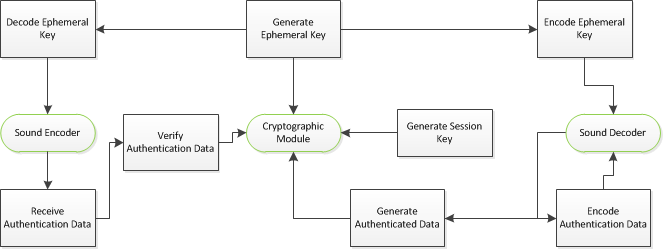
\includegraphics[width=1\textwidth]{img/architecture}
	\caption{Application architecture.}
\end{figure}

\subsection{Cryptography library}

Exist few of cryptography libraries which are written in Java (e.g. javax.crypto, BouncyCastle), but we wanted to create cryptography module which is independent of the platform. The choice fell on CryptoPP. It is free, open source cryptography library written in C++. The library is objectives and very easy to use. Ensures symmetric and asymmetric cryptography along with signatures and secure hash function. Is used by such companies as Microsoft or Symantec.

\subsection{Design pattern}

Application architecture base on Model-View-Controller pattern. As model is included whole cryptographic module, controller receive and send data to appropriate places and view is responsible for sending and receiving data associated with AMA protocol. 

\begin{figure}[H]
	\centering
	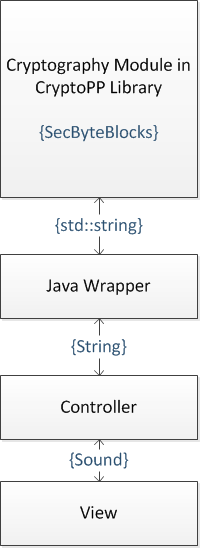
\includegraphics[width=0.3\textwidth]{img/Design}
	\caption{Design pattern.}
\end{figure}

\subsection{NIST recommendation for security parameters}

NIST recommends using 3072 bit length keys to ensure low probability of calculating discrete logarithm. This length is set as default in CryptoPP, however in our prototype we are using 1024 bit. It is caused by duration of sending data by sound. Now, sending 1024 bit length keys take some time and for needs of presentation we decided to stay with this length. For more information please check \cite{NIST}.

\subsection{Shared cryptographic module}
Cryptographic module is designed in such way that it will be easy to use it on different platforms. Application treat it as a black box where are exchanging strings with data. Implementation is made in C++ based on DiffieHellman and Authenticated-DiffieHellman classes from CryptoPP library. It performs following cryptographic operation:

\begin{itemize}
\item Modular exponentiation
\item Long term and ephemeral key generation (Diffie-Helman)
\item Certificate generation and verification
\item Secure hashing (SHA1)
\item Symmetric encryption (AES)
\end{itemize}

Core of this module is class MututalAuthenticationChip. It is responsible for inputting, preparing and outputting data to Application. All sensitive data is kept internally using secure byte blocks. Messages generated in the protocol are converted to strings.
For group arithmetic operations and modular exponentiation we use build in Integer class provided by the library. 

\vspace{5mm}

The overall implementation tightly follows the protocol specification and the only overhead is connected with conversions to provide compatibility with the rest of the application.
\lstset{language=C++,caption={Example of CryptoPP usage for ephemeral key generation.}}
\begin{lstlisting}
void KeyGenerator::GenerateEphemeralKeyPair(CryptoPP::RandomNumberGenerator &rng, byte *privateKey, byte *publicKey) const
{
    Integer a = Integer(rng, keySize);
    byte *aEncoded = new byte[keySize];
    a.Encode(aEncoded, keySize);
    privateKey = HashClass::getSHA1(aEncoded, keySize);
    CryptoPP::Integer exponent(privateKey, keySize);
    CryptoPP::Integer cA = a_exp_b_mod_c(g, exponent, p);   //ca = g^H(a)
    cA.Encode(publicKey, keySize);
}
\end{lstlisting}

\subsection{Java Native Interface - C++ Wrapper}

To be able to use cryptographic part written in C++ in Android, we had to create C++ wrappers using JNI (Java Native Interface) \cite{JNI}. Main class which communicate with C++ code has native methods, for which, after appropriate compilation, was created MACWrapper.h where definition of methods looks like below.

\lstset{language=C++,caption={Example of JNI usage for method definition.}}
\begin{lstlisting}
/*
 * Class:     com_example_androidake_MutualAuthenticateChip
 * Method:    prepareMACCPP
 * Signature: (Z)V
 */
JNIEXPORT void JNICALL Java_com_example_androidake_MutualAuthenticateChip_prepareMACCPP
  (JNIEnv *, jobject, jboolean);
\end{lstlisting}

Implementations of methods are in MACWrapper.cpp. There are made conversion from C++ data type to Java data type and vice versa.

\lstset{language=C++,caption={Example of JNI usage for method implementation.}}
\begin{lstlisting}
JNIEXPORT void JNICALL Java_com_example_androidake_MutualAuthenticateChip_prepareMACCPP
(JNIEnv *env, jobject thisObj, jboolean jinit) {
	bool init = jinit;
	if(init == true) {
		mac = new MutualAuthenticationChip(init);
	} else {
		mac_B = new MutualAuthenticationChip(init);
	}
};
\end{lstlisting}

\subsection{Base64}

One of the biggest problem was decided in what representation data should be sending. First choice was standard binary representation with 0 and 1. During creation of sound channel we have found that sending one ephemeral key, which has 1024 bits will take too long. So we decided to reduce sending data using Base64 conversion. Six bits are transform to one of the 64 defined signs. Hence, instead of sending 1024 sings we send just about 172. Data which come from cryptographic module are in Hexadecimal representation. To converse we have used library created by Robert Harder \cite{base_64}. 

\begin{lstlisting}[caption={Example of code converting from Hex String to Base64 String}]
public static String fromHexToBase64(byte[] hex_byte) {
	String hex_str = ConverterJava.ByteToString(hex_byte);
	byte[] decodedHex = null;
	try {
		decodedHex = Hex.decodeHex(hex_str.substring(0,
				hex_str.length() - 1).toCharArray());
	} catch (DecoderException e) {
		e.printStackTrace();
	}
	String encodedHexB64 = Base64.encodeBytes(decodedHex);
	return encodedHexB64;
}
\end{lstlisting}

\subsection{Sound channel}

Sound channel was one of the most difficult part during creation of application. One of the reason was inaccessibility of library whereby we could transform received sound data to cryptographic data. Whole process of analysis received data had to be created from beginning. At beginning we had doubt about sensitivity and precision of speaker and microphone in mobile devices, especially when we wanted to use ultrasonic waves which could be hard to interpreter. Fortunately, doubts were dispelled after first testing of this channel. Results of working will be describe in Test section. Here we focus on principle of operation.

\subsubsection{Generating sound wave}

Class responsible for generating sound wave get data presented in Base64 (Check section with Base64). Every character A-Z, a-z, 0-9, + and / is mapped to one of the 64 frequencies.

A = 10 kHz,

B = 10,15 kHz,

C = 10,3 kHz,

...

. = 19,55 kHz


Additional two characters "," and "." represent begin of data and end of data. Sample rate is 44,1 kHz. Every character is sending by 30 ms, which means that for each pitch is needed 1323 samples. To create sinus wave each sample for $ i \in (0,1322) $ is calculating by formula:
\begin{center}
$F(i) = \sin($ $f \ast PI \ast 2 \ast i  \over 44 100 $ $)$
\end{center}
where $f$ is the target frequency.
These samples are processed by AudioTrack library to sound using PCM encoding. 


\subsubsection{Receiving sound}

Retrieving sound is more complicated than sending. In separate process, using AudioRecord library, in every 15 milliseconds (if sending of one character takes 30 ms), are taken samples and then, as one buffer, are appended to array of buffers. Separate process, in the same time, takes first buffer from array and analyses it. 

\vspace{5mm}

At this moment, the samples are as short integer values which represent sound in time domain (sinusoid). To check in which frequency was received sound is needed to convert the sampled function from time domain to the frequency domain. We used to this Discrete Transform Fourier. Library which we have chosen to run DFT is \cite{minim_dft}. 

\vspace{5mm}

Before change of domain, we need to window samples, using Hanning windowing. Thereby, chart in frequency domain is more readable and is easier to find the place with the highest pitch. Windowed samples are put into DFT method and on the output we have result in frequency domain. The effect on the graph looks like at \ref{fig:F2}.


\begin{figure}[H]
	\centering
	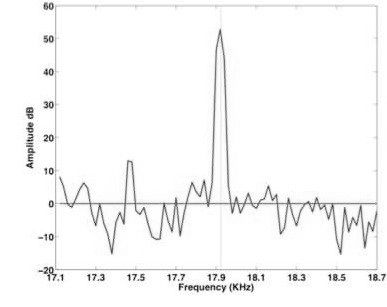
\includegraphics[width=0.45\textwidth]{img/peaks_1}
	\label{fig:F2}
\end{figure}



Now, algorithm tries to find the highest place in the output. The reason of getting data in two times shorter time than sending one character is that, in one buffer can be two frequencies. In the worst case, algorithm can find one frequency in three buffers in a row, even if in first and third buffer was also another frequency, but because of lower sound intensity or less samples representing this frequency, would not be found as a highest pitch. Dividing time of receiving by two ensure that always, at least once, expected frequency will be registered. If he finds pitch with amplitude higher than 50, for frequency lower than 14 kHz, or 10 for higher than 14 kHz (this different follows from the smaller volume for the higher frequency by hardware limitation) is checked whether caught frequency is in our dictionary (with margin of error + - 50 Hz). 


\begin{figure}[H]
	\centering
	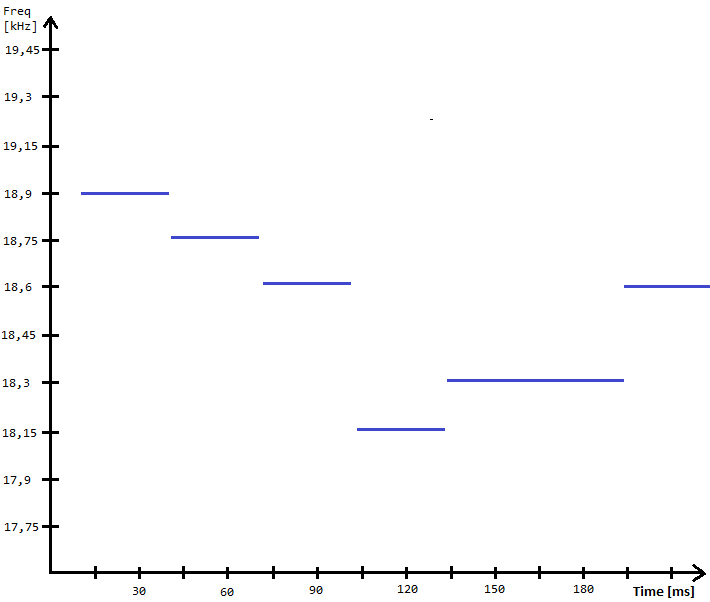
\includegraphics[width=0.70\textwidth]{img/receiving}
	\caption{Figure show received frequencies in time.}
\end{figure}

Caught value is put to the memory and wait for the next result. If current frequency is different than before we change the previous frequency to one of the 64 signs. Otherwise we increment the counter. If counter gain value three (maximal number of occurrences on received character in three further buffers), counter is reset and return adequate character.


\section{Tests}
To all tests was used two devices: LG Swift L9 with system Android 4.1.2 and tablet Samsung GALAXY Tab 2 with Android 4.2.2. 

\subsection{Receiving data in sound channel}
During tests we have focused on below factors:
\begin{itemize}
\item Distance between devices.
\item Position of devices terms of placement of speaker and microphone.
\item Distance between chosen frequencies.
\item Working during sounds in the background.
\item Sending characters in shorter time than 30 ms.
\end{itemize}

Firstly, we have tested distance between chosen frequencies. Every character from Base64 coding is mapped to appropriate frequency. The smaller distance then is possible to use higher frequencies. We have choose three spaces:
\begin{itemize}
\item 150 Hz. The lowest frequency 10,5 kHz, the highest - 20,25 kHz.
\item 130 Hz. The lowest frequency 11,8 kHz, the highest - 20,25 kHz.
\item 100 Hz. The lowest frequency 13,8 kHz, the highest - 20,3 kHz.
\item 100 Hz. The lowest frequency 14 kHz, the highest - 20,5 kHz.
\item 100 Hz. The lowest frequency 14,3 kHz, the highest - 20,8 kHz.
\end{itemize}
We did not want to go below 10 kHz and higher frequency than 20,5 is hard to detect for mobile phone (especially for LG). Distance 100 Hz is the smallest to test because of implemented algorithm (margin of error is + - 50 Hz). During the tests, proved to be that for almost every test cases, protocol was successful in 70\%. Except the last one which always end by failure. Character which represent end of sending data has always the highest frequency. In this case it was 20,8 kHz. Only LG Swift cannot registry that frequency - Samsung dealt with it flawlessly.

\vspace{5mm}

There are several reason why the result was not 100\%. Sometimes, if we send, for example, frequency 20 kHz then second device receive it as 19,9. It can be caused by some distortion on the microphone or even on the speaker. What happened was that the speaker make sound different than usual and then was needed restart of device. Sometimes it is sufficient that one of the device froze on some milliseconds and then receiving device lose some characters. 

\vspace{5mm}

Measure of allowed distance between devices we have started with stick microphone from LG with speaker from Samsung. This gave us the best results. Received amplitude was the biggest, hence easier, for algorithm, was to find interesting for us frequency. Then we increased distance to 2 cm. In this case results were also good. Sessions keys were established almost every time. Problem was started increasing distance to 6 cm. Higher frequencies were not registered by microphone. Placing the devices parallel the protocol always end by failure. The LG was not able to gain all frequencies in such way. Samsung again has been receiving data without problems. 

\vspace{5mm}

The next test rely on checking influence of background sound. As we know, from the previous test, the best results were when devices were close to each other (maximal 2 cm from each other), so we have tested it in such position. At beginning we have checked it at the University during the break between lectures. A lot of students was talking and laughing but even this, did not interfere with protocol. Almost every attempt was ended with success. Then we have used third device which was generating constantly chosen frequency. We have put this device very close to the participants. First disturbing frequency was 8 kHz. Because of that bandwidth is from 10,5 to 20,25 we have suspected that 8 kHz will not cause the problem and we was right. Algorithm analyzing data has not mistaken. The problem was just after increasing disturbing frequency above 10,5 kHz, but was needed to stick speaker of this device to microphone of protocol participant. Otherwise, the protocol always ends with success. 


\subsection{Summary}
%%%%%%%%%%%%%%%%%%%%%%%%%%%%%%%%%%%%%%%%%%%%%%%%%%%%%%%%%%%%%%%%%%%%%%%%%%%%%%
%%%%%%%%%%%%%%%%%%%%%%%%%%%%%%% BIBLIOGRAFIA %%%%%%%%%%%%%%%%%%%%%%%%%%%%%%%%%
%%%%%%%%%%%%%%%%%%%%%%%%%%%%%%%%%%%%%%%%%%%%%%%%%%%%%%%%%%%%%%%%%%%%%%%%%%%%%%


\bibliographystyle{plain}

\bibliography{AKESound}


\end{document}